\documentclass[11pt,a4paper]{article}

% --- packages ---
\usepackage[margin=1in]{geometry}
\usepackage{graphicx}
\usepackage{booktabs}
\usepackage{amsmath}
\usepackage{amssymb}
\usepackage{hyperref}
\usepackage{natbib}
\usepackage{xcolor}
\usepackage{enumitem}
\usepackage{caption}
\usepackage{subcaption}
\usepackage{microtype}
\usepackage{url}
\usepackage{setspace}

\hypersetup{
  colorlinks=true,
  linkcolor=blue!50!black,
  citecolor=blue!50!black,
  urlcolor=blue!60!black
}

\title{Agentic Retrieval Systems:\\
A Reproducible Framework for Comparing Conventional RAG,\\
Iterative, and Multi-Agent Retrieval}

\author{
Ben Karlsberg\\
Georgia Institute of Technology\\
\texttt{bkarlsberg3@gatech.edu}
}

\date{}

\begin{document}
\maketitle

\begin{abstract}
Retrieval-augmented generation (RAG) systems increasingly incorporate iterative
and multi-agent control loops, yet fair comparisons across architectures remain
difficult: implementations differ in corpora, budgets, traces, and metrics.
We present \textbf{Agentic Retrieval Systems (ARS)}, an open-source evaluation
framework that places conventional retrieve-once RAG, a budgeted single-agent
iterative retriever, and a role-separated multi-agent pipeline under a shared
corpus, model interface, metric suite, and hard budget regime.
ARS records structured JSONL traces (queries, retrieved documents, routing
decisions, stop reasons, and token accounting) and supports budget-matched
modes (\texttt{equal\_retrieval}, \texttt{equal\_token}, unconstrained).
We validate the harness offline with a deterministic heuristic model and
checked-in mini fixtures ($n{=}13$ examples, 24 passages).
On this synthetic setup, answer quality is matched across architectures
(EM\,$\approx$\,0.85, F1\,$\approx$\,0.81, abstention correctness\,$=$\,1.0),
while process cost increases monotonically:
RAG $\ll$ single-agent $\ll$ multi-agent in model calls and tokens.
These results are \emph{not} frontier LLM benchmarks; they demonstrate
harness correctness and quantify coordination overhead under controlled
conditions.
ARS is released at
\url{https://github.com/benkarlsberg/Agentic-Retrieval-Systems}
to support reproducible comparisons as live models and larger public datasets
are introduced via adapters.
\end{abstract}

\section{Introduction}
\label{sec:intro}

Open-domain question answering and related knowledge-intensive tasks
increasingly rely on retrieval-augmented generation
\citep{lewis2020rag,karpukhin2020dpr,gao2023ragsurvey}.
Beyond the classical retrieve-once pattern, recent systems interleave
retrieval with reasoning \citep{trivedi2023ircot,jiang2023flare,yao2023react},
reflect on evidence quality \citep{asai2023selfrag}, and route queries by
complexity \citep{jeong2024adaptiverag}.
In parallel, multi-agent designs decompose planning, retrieval, critique, and
synthesis across specialized roles.
These agentic designs promise better coverage on multi-hop and multi-passage
questions, but they also introduce coordination overhead: extra model calls,
duplicate retrievals, longer traces, and higher latency.

A practical obstacle for research and engineering is \emph{fair comparison}.
Published systems rarely share identical corpora, budget caps, logging
schemas, and metric definitions, so observed quality gaps may confound
architecture with implementation choices.
We argue that progress on agentic retrieval requires a harness that holds
those factors fixed and makes process cost as first-class as answer quality.

\paragraph{Research questions.}
We organize the framework around four questions:
\begin{enumerate}[leftmargin=*,itemsep=2pt]
  \item[\textbf{RQ1}] Under matched retrieval or token budgets, does bounded
    iterative retrieval improve answer quality over retrieve-once RAG on
    multi-hop / multi-passage items?
  \item[\textbf{RQ2}] Does role-separated multi-agent retrieval improve
    evidence coverage and citation fidelity enough to justify coordination
    overhead?
  \item[\textbf{RQ3}] How do architectures differ on unanswerable and
    ambiguous questions (abstention vs.\ false answers)?
  \item[\textbf{RQ4}] How sensitive are architecture rankings to sparse
    (BM25), dense, and hybrid retrieval under a fixed corpus?
\end{enumerate}

\paragraph{Contributions.}
\begin{enumerate}[leftmargin=*,itemsep=2pt]
  \item A reproducible systems framework comparing three architectures
    (conventional RAG, bounded single-agent, multi-agent) with shared
    retrieval, budgets, metrics, and JSONL tracing.
  \item Explicit budget-matched comparison modes and first-class
    termination reasons, enabling efficiency-aware evaluation.
  \item An offline-fixture validation study ($n{=}13$) with
    \texttt{DeterministicModel}, confirming pipeline correctness and
    quantifying process overhead when quality is matched.
  \item An open-source release with adapters for larger public datasets
    (user-supplied local files) and optional live model backends.
\end{enumerate}

\paragraph{Scope.}
This paper is primarily a \emph{systems and evaluation framework} paper with
a small synthetic validation study.
Checked-in numbers use a heuristic model and mini fixtures; they must not be
read as HotpotQA/Natural Questions leaderboard results or claims of
state-of-the-art answer quality for agentic systems.

\section{Related Work}
\label{sec:related}

\paragraph{Retrieve-and-read and dense retrieval.}
Classical open-domain QA pipelines retrieve passages and then read them for
answers \citep{chen2017drqa}.
Dense Passage Retrieval \citep{karpukhin2020dpr} and RAG
\citep{lewis2020rag} popularized end-to-end neural retrieval with generation.
Sparse baselines such as BM25 remain strong and widely used
\citep{robertson2009bm25}.
Hybrid fusion (e.g., reciprocal rank fusion) often combines sparse and dense
signals \citep{cormack2009rrf}.

\paragraph{Iterative and adaptive retrieval.}
IRCoT interleaves retrieval with chain-of-thought reasoning for multi-step
questions \citep{trivedi2023ircot}.
FLARE triggers retrieval when generation confidence is low
\citep{jiang2023flare}.
Self-RAG trains models to decide when to retrieve and how to critique
evidence \citep{asai2023selfrag}.
Adaptive-RAG routes queries by estimated complexity
\citep{jeong2024adaptiverag}.
ReAct and related tool-using agents couple reasoning with actions such as
search \citep{yao2023react,schick2023toolformer,press2023selfask}.
ARS does not claim a new retrieval policy; it provides a controlled substrate
on which such policies can be compared under matched budgets.

\paragraph{Multi-hop benchmarks.}
HotpotQA \citep{yang2018hotpotqa}, Natural Questions
\citep{kwiatkowski2019nq}, and 2WikiMultiHopQA \citep{ho2020twowiki}
remain standard evaluation resources.
ARS ships adapters that load \emph{user-provided} local copies; it does not
redistribute those datasets, and this paper reports no leaderboard numbers
on them.

\paragraph{Evaluation methodology.}
Surveys of RAG emphasize the need for systematic metrics spanning answer
quality, retrieval, faithfulness, and cost \citep{gao2023ragsurvey}.
ARS contributes a concrete harness: typed schemas, paired bootstrap
confidence intervals \citep{efron1993bootstrap}, and auditable traces.

\section{Framework Design}
\label{sec:design}

\subsection{Architectures}
\label{sec:arch}

ARS implements three runners that share the same corpus, retriever factory,
model client interface, budget controller, and metric suite.

\paragraph{A --- Conventional RAG.}
A single retrieval call returns \texttt{top\_k} passages; one generation
call produces the answer.
This is the retrieve-once baseline corresponding to classical RAG.

\paragraph{B --- Bounded single-agent.}
A decision loop may \emph{retrieve}, \emph{reformulate} the query, or
\emph{stop}.
Hard caps on steps, model calls, retrieval calls, documents, and tokens
prevent unbounded loops.
Stop reasons (e.g., answer ready, budget exhausted) are logged as first-class
events.

\paragraph{C --- Multi-agent.}
A planner decomposes the information need; role-specialized retrievers issue
queries; a critic assesses evidence sufficiency; a synthesizer produces the
final answer.
Coordination messages are recorded in traces so overhead is measurable
rather than implicit.

\subsection{Shared retrieval stack}
Retrievers include BM25 (with a pure-Python fallback), dense retrieval over
fixture embeddings (hashing-based for offline use, not a trained dual
encoder), hybrid RRF fusion, and an optional lexical reranker.
Architecture rankings under RQ4 are therefore attributable to retrieval
\emph{modality} rather than divergent corpora.

\subsection{Budgets and comparison modes}
Default budgets specify limits on steps, model calls, documents, tokens,
retrieval calls, and \texttt{top\_k}.
Comparison modes include:
\begin{itemize}[leftmargin=*,itemsep=1pt]
  \item \texttt{equal\_retrieval}: matched retrieval-call / document budgets
    (RAG remains a single retrieve);
  \item \texttt{equal\_token}: matched token budgets;
  \item \texttt{unconstrained}: per-architecture defaults, still hard-capped.
\end{itemize}
These modes operationalize fair comparison for RQ1--RQ2.

\subsection{Tracing}
Every example emits JSONL events covering reformulated queries, retrieved
document IDs and scores, routing actions, model/token accounting, latency,
estimated cost, and termination reason.
An HTML trace viewer supports qualitative audit.
Prompt text may be hashed in traces to reduce accidental leakage of
sensitive content in live runs.

\subsection{Metrics}
ARS reports:
\begin{itemize}[leftmargin=*,itemsep=1pt]
  \item \textbf{Answer:} exact match (EM), token F1, lexical similarity;
  \item \textbf{Retrieval:} recall@$k$, mean reciprocal rank (MRR);
  \item \textbf{Citations:} precision/recall against gold document IDs when
    available;
  \item \textbf{Abstention:} correctness on unanswerable items;
  \item \textbf{Efficiency:} latency, model calls, retrieval calls, tokens,
    unique vs.\ duplicate passages, config-based cost estimates.
\end{itemize}
Paired bootstrap confidence intervals on per-example metric deltas support
architecture comparisons on shared IDs.

\subsection{Model interface}
A provider-neutral client supports (i)~a \texttt{DeterministicModel} for
offline CI and fixture validation, and (ii)~optional OpenAI-compatible live
backends via environment configuration.
Live keys are never committed; live results must be labeled separately from
fixture baselines.

\section{Experimental Setup}
\label{sec:setup}

\subsection{Offline fixtures}
The checked-in evaluation uses:
\begin{itemize}[leftmargin=*,itemsep=1pt]
  \item Corpus: \texttt{fixtures/corpus/mini\_wiki.jsonl} (24 passages);
  \item Dataset: \texttt{fixtures/datasets/mini\_eval.jsonl} ($n{=}13$
    questions spanning single-hop, multi-hop/multi-passage, and
    unanswerable items);
  \item Model: \texttt{DeterministicModel} (\texttt{deterministic-v1}), a
    keyword/heuristic answerer over retrieved context;
  \item Retrieval: BM25, \texttt{top\_k}\,$=$\,5;
  \item Seed: 42;
  \item Mode: \texttt{unconstrained} (primary table); equal-retrieval mode
    also exercised.
\end{itemize}
\textbf{Label:} all reported numbers are \emph{offline-fixture / synthetic
validation of the harness}, not frontier LLM evaluations.

\subsection{DeterministicModel policy}
The mock model extracts answers from retrieved passages with fixed
heuristics and question gating.
Consequently, when retrieval surface form is similar, architectures tend to
\emph{match} on EM/F1; differences appear in control flow and cost.
This is intentional for validating wiring, budgets, and traces without API
keys.

\subsection{Configs and reproduction}
Primary config:
\texttt{configs/experiments/offline\_fixture\_compare.yaml}.
Budget-matched configs include
\texttt{equal\_retrieval.yaml} and \texttt{equal\_token.yaml}.
Ten ablation YAML files document planned studies (critic/planner ablations,
hybrid/dense retrieval, \texttt{top\_k}, strict budgets, reformulation off,
reranker).
Reproduction:
\begin{verbatim}
pip install -e ".[dev]"
python scripts/run_experiment.py \
  --config configs/experiments/offline_fixture_compare.yaml
python scripts/generate_report.py --run-dir results/runs/latest
\end{verbatim}
Artifacts include per-architecture summaries, comparison tables, plots, and
full traces under \texttt{results/}.

\section{Results}
\label{sec:results}

Table~\ref{tab:main} reports the primary offline-fixture comparison
(unconstrained BM25, seed 42, $n{=}13$).
Figure~\ref{fig:tradeoff} visualizes per-example F1 against token cost;
Figures~\ref{fig:em}--\ref{fig:f1} summarize mean EM and F1.

\begin{table}[t]
\centering
\caption{Offline-fixture validation ($n{=}13$, DeterministicModel, BM25,
unconstrained, seed 42). Quality is matched; process cost increases with
agentic complexity. EM/F1 rounded to three decimals; tokens are means.}
\label{tab:main}
\begin{tabular}{lcccccc}
\toprule
Architecture & EM & F1 & Abst.\ corr. &
  Avg.\ model & Avg.\ retr. & Avg.\ tokens \\
\midrule
RAG            & 0.846 & 0.810 & 1.000 & 1.00 & 1.00 & $\sim$295 \\
Single-agent   & 0.846 & 0.810 & 1.000 & 3.00 & 1.00 & $\sim$654 \\
Multi-agent    & 0.846 & 0.810 & 1.000 & 4.31 & 2.31 & $\sim$1626 \\
\bottomrule
\end{tabular}
\end{table}

\begin{figure}[t]
\centering
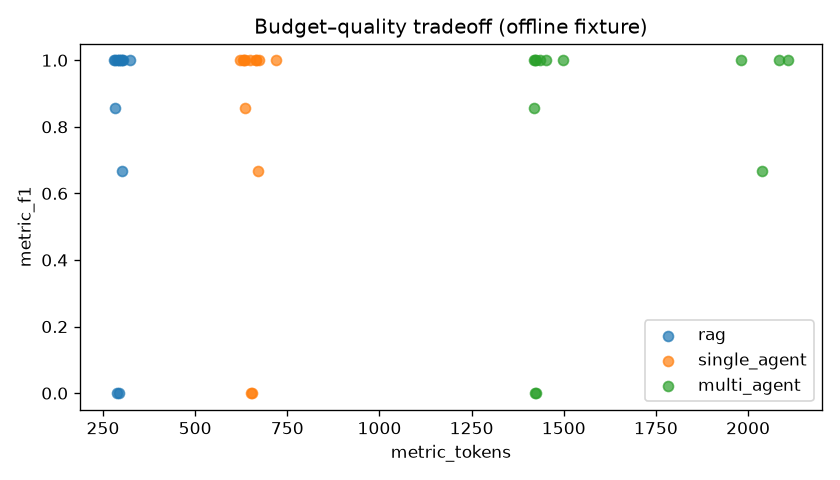
\includegraphics[width=0.85\linewidth]{figures/offline_fixture_tradeoff.png}
\caption{Budget--quality tradeoff on the offline fixture (per-example F1 vs.\
tokens). Architectures share similar F1 mass near 1.0 with a common failure
at F1\,$=$\,0; multi-agent occupies a higher token regime. This plot
illustrates process overhead under matched heuristic quality---not a live
LLM ranking.}
\label{fig:tradeoff}
\end{figure}

\begin{figure}[t]
\centering
\begin{subfigure}[t]{0.48\linewidth}
  \centering
  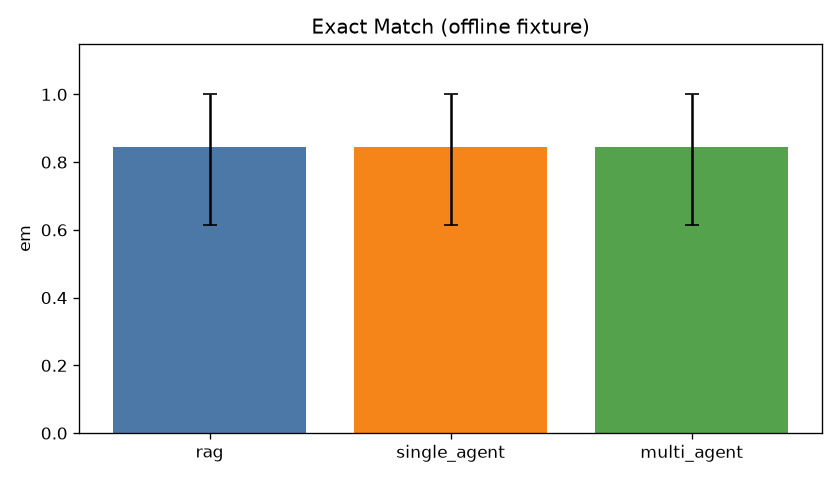
\includegraphics[width=\linewidth]{figures/offline_fixture_em.png}
  \caption{Mean EM.}
  \label{fig:em}
\end{subfigure}
\begin{subfigure}[t]{0.48\linewidth}
  \centering
  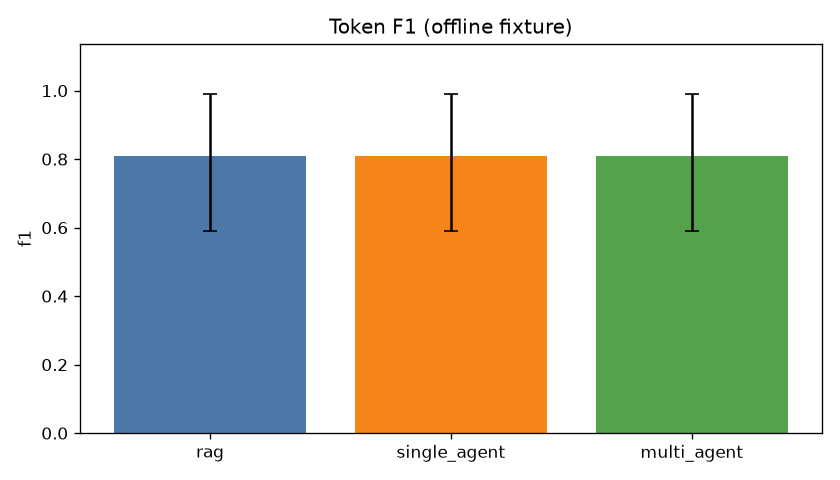
\includegraphics[width=\linewidth]{figures/offline_fixture_f1.png}
  \caption{Mean F1.}
  \label{fig:f1}
\end{subfigure}
\caption{Offline-fixture answer metrics by architecture. Bars are essentially
identical; the evaluation signal for this run is efficiency, not quality
separation.}
\label{fig:em_f1}
\end{figure}

\paragraph{Quality.}
EM ($0.846$), F1 ($0.810$), and abstention correctness ($1.0$) are identical
across architectures on this fixture after question-gated mock answering.
Bootstrap 95\% intervals are wide (as expected for $n{=}13$).
Eleven of thirteen answerable-or-partial items score as successful under the
EM/F1 thresholds used in reporting; both unanswerable items yield correct
abstention for all three runners.

\paragraph{Efficiency (primary signal).}
Average model calls rise from $1.00$ (RAG) to $3.00$ (single-agent) to
$4.31$ (multi-agent).
Average tokens rise from $\sim$295 to $\sim$654 to $\sim$1626.
Multi-agent also issues more retrieval calls ($2.31$ vs.\ $1.00$) and logs
coordination messages.
Thus the harness recovers the designed cost ordering
RAG $\ll$ single-agent $\ll$ multi-agent when answer quality is held
approximately fixed by the deterministic policy.

\paragraph{Equal-retrieval mode.}
An equal-retrieval budget run completed successfully without API keys,
exercising matched retrieval caps while preserving shared metrics and
traces.
This confirms that budget modes are operational for future live-model
comparisons under RQ1.

\paragraph{What we do not claim.}
We do not claim that agentic architectures outperform RAG on frontier LLMs,
nor do we report HotpotQA/NQ scores.
Fixture equality of EM/F1 is expected under a shared heuristic answerer; it
is evidence that evaluation plumbing is consistent, not that agentic
complexity is useless in general.

\section{Discussion}
\label{sec:discussion}

\paragraph{What fixture runs show.}
Offline runs validate that (i)~all three architectures execute end-to-end,
(ii)~hard budgets and stop reasons are enforceable, (iii)~traces are complete
enough for audit, (iv)~metrics and paired bootstrap utilities are wired, and
(v)~process overhead is measurable and ordered as designed.

\paragraph{What they do not show.}
They do not establish absolute quality of production LLMs, production latency
distributions, or architecture rankings on full multi-hop benchmarks.
Statistical power is limited by $n{=}13$.

\paragraph{When agentic complexity may help.}
Under live models, iterative reformulation and multi-agent role separation
are hypothesized to help when: evidence is split across passages (multi-hop);
one-shot BM25 misses a second hop; citation fidelity and evidence recall
matter more than token cost; or unanswerable questions require explicit
abstention policies beyond naive generation.
ARS is designed so those hypotheses can be tested under
\texttt{equal\_retrieval} / \texttt{equal\_token} with paired bootstrap
deltas---once a live backend and larger stratified samples are configured.

\paragraph{Systems insights.}
Making budgets and stop reasons first-class prevents silent unbounded agent
loops.
Shared retrieval and schemas reduce confounds.
Treating coordination messages and duplicate passages as metrics reframes
``multi-agent benefit'' as an explicit cost--benefit question (RQ2).

\section{Limitations}
\label{sec:limitations}

\begin{itemize}[leftmargin=*,itemsep=2pt]
  \item \textbf{Synthetic validation only.} Checked-in results use
    \texttt{DeterministicModel} and mini fixtures; they are not frontier
    benchmarks.
  \item \textbf{Small $n$.} Wide confidence intervals; rankings are not
    statistically decisive.
  \item \textbf{Dense retrieval.} Fixture dense embeddings use hashing, not
    trained dual encoders such as DPR \citep{karpukhin2020dpr}.
  \item \textbf{Ablation toggles.} Ten ablation configs are present; some
    behavioral switches (e.g., hard skip-critic) remain extension points.
  \item \textbf{Cost estimates.} USD figures in configs are timestamped
    estimates, not live billing.
  \item \textbf{Dataset redistribution.} HotpotQA/NQ/2Wiki adapters require
    user-provided local files; no leaderboard results are reported here.
\end{itemize}

\section{Conclusion and Future Work}
\label{sec:conclusion}

We introduced Agentic Retrieval Systems (ARS), a reproducible framework for
comparing conventional RAG, bounded iterative retrieval, and multi-agent
retrieval under shared corpora, budgets, traces, and metrics.
An offline-fixture study confirms harness correctness and shows matched
heuristic quality with clearly increasing coordination and token cost as
architectures become more agentic.
We release the code openly to support controlled follow-on experiments.

\paragraph{Future work.}
(1)~Live OpenAI-compatible models on stratified samples of 100--200
multi-hop-style items under equal-retrieval and equal-token modes;
(2)~full behavioral enforcement of ablation switches;
(3)~learned rerankers and trained dense encoders;
(4)~error taxonomies mined from traces (query drift, duplicate retrieval,
premature stop);
(5)~larger public datasets via existing adapters with clear separation of
live results from fixture baselines.

\section*{Acknowledgments}
The author thanks the open-source community for tools used in retrieval and
evaluation infrastructure.
Code is available at
\url{https://github.com/benkarlsberg/Agentic-Retrieval-Systems}
under the MIT license.

\bibliographystyle{plainnat}
\bibliography{references}

\end{document}
